\section{Jasmine}
Um schon während der Entwicklung eine gute Qualität des Quelltextes anzustreben, ist der Einsatz von einem Testing-Framework sinnvoll. Die Wahl fällt auf Jasmine, da es eine einfache Implementierung ermöglicht sowie clientseitig ohne einen Server funktioniert. 

Jasmine ist ein verhaltensorientiertes Entwicklungsframework zum Testen von JavaScript-Code. Es hängt nicht von anderen JavaScript-Frameworks ab. Es benötigt kein DOM. Und es hat eine saubere, explizite Syntax, so dass man problemlos Tests schreiben kann \cite{jasmine}. Zusätzlich folgt Jasmine der BDD-Prozedur (Behavior Driven Development), um sicherzustellen, dass jede Zeile der JavaScript-Anweisung ordnungsgemäß Unit-getestet ist. Durch das Befolgen der BDD-Prozedur bietet Jasmine eine kleine Syntax, um die kleinste Einheit der gesamten Anwendung zu testen, anstatt sie als Ganzes zu testen.  

Im Folgenden sind die Vorteile der Verwendung von Jasmine gegenüber anderen verfügbaren JavaScript-Test-Frameworks aufgeführt \cite{jasmineTutorial}.
\begin{itemize}
\item	Jasmine ist von keinem anderen JavaScript-Framework abhängig.
\item	Jasmine benötigt kein DOM.
\item	Die gesamte im Jasmine-Framework verwendete Syntax ist sauber und offensichtlich.
\item	Jasmine wird stark von Rspec, JS Spec und Jspec beeinflusst.
\item	Jasmine ist ein Open-Source-Framework und leicht verfügbar in verschiedenen Versionen wie Stand-alone, Ruby-Juwel, Node.js, etc.
\end{itemize}



\subsection{Wie benutzt man Jasmin?}
%Man kann Jasmine unter \url{https://github.com/jasmine/jasmine/releases} herunterladen.
Jasmine ist sehr einfach in jeder Art von Entwicklungsmethodik zu implementieren. Alles, was man herunterladen muss, ist die Standalone-Bibliotheksdateien von der offiziellen Website \url{https://github.com/jasmine/jasmine/releases}. Dieses implementiert man gleich in seiner Anwendung. Nach dem Entpacken der Jasmine-Bibliothek muss man den Entpacker-Ordner in den Unit-Tests-Ordner der erstellten Anwendung einfügen. Der Entpacker-Ordner umfasst:
\begin{figure}[ !h] \centering
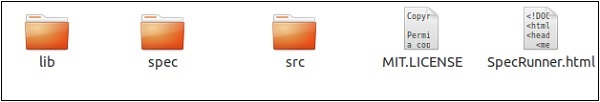
\includegraphics[width=1.0\textwidth]{jasmineLib}
\caption[Jasmine-Bibliotheksdateien]{Jasmine Standalone-Bibliotheksdateien\\ Quelle: \url{https://www.tutorialspoint.com/jasminejs/jasminejs_overview.htm}}\label{fig:jasmineLib}
\end{figure}
\begin{itemize}
\item	\textit{Lib:} enthält Quellcode für das Framework.
\item	\textit{Spec}: enthält Code für seine Tests
\item	\textit{Src:} enthält Quellcode für seine Anwendung
\item 	\textit{SpecRunner.html:} ist eine Seite, die man Tests ausführt.
%Man können Verweise auf seine Spezifikationen (Tests) und den Quellcode für die Anwendung sehen, die Sie testen möchten. Es ist also nicht notwendig, den Code in den Ordner \textit{``src''} zu kopieren. Man kann einfach Ihre Spezifikationen in diese Datei einbinden.
\end{itemize}
Dieses Paket enthält auch ein kleines Beispiel, das nützlich sein könnte.

\subsection{Wie man mit Jasmine JS Tests prüft?}
Ein einfaches Beispiel für JavaScript-Tests von Jasmine sieht folgendermaßen aus:
%https://www.apriorit.com/dev-blog/372-testing-javascript-with-jasmine
\begin{lstlisting}[language=JavaScript,basicstyle=\scriptsize]
describe("App", function () {
    describe("foo", function () {
        it("should return bar", function () {
            expect(App.foo()).toEqual("bar");
        });
    });
});

var App = {
    foo: function() {
        return "bar123";
    }
};
\end{lstlisting}

Im obigen Beispiel wird \textit{App.foo(}) durch die Suite \textit{``App''} mit Matcher \textit{.toEqual} getestet. 

%https://www.htmlgoodies.com/beyond/javascript/testing-javascript-using-the-jasmine-framework.html
Eine Suite stellt eine Reihe von verwandten Tests dar. Jede Suite enthält wiederum eine Reihe von Erwartungen, die die Ergebnisse des Tests - den tatsächlichen Wert - mit dem erwarteten Wert vergleichen. Eine Suite wird durch Aufrufen der Funktion \textit{describe()} definiert. Es benötigt zwei Parameter: den Namen der Suite und die Funktion, die die Aufrufe der Erwartungs-Methoden enthält. Diese werden mit der Methode \textit{it()} definiert. Wie \textit{describe()} akzeptiert \textit{it()} auch einen Namen und einen Funktionsparameter. Der Funktionsparameter \textit{it()} kann Variablen und einen oder mehrere Aufrufe der \textit{expect()} enthalten. In Verbindung mit einer Matcher-Funktion führen diese die Aufgabe durch, die Ist- und Erwartungswerte zu vergleichen. Jeder Matcher implementiert einen booleschen Vergleich zwischen dem tatsächlichen Wert und dem erwarteten Wert. Es ist verantwortlich für die Berichterstattung an Jasmine, wenn die Erwartung wahr oder falsch ist. Jasmine wird dann die Spezifikation bestehen oder nicht bestehen.

Jeder Matcher kann eine negative Assertion auswerten, indem er den Call \textit{expect()} mit einem \textit{``not''} vor dem Aufruf des Matcher verkettet. Jasmine bietet eine große Auswahl an Matching-Tools. Die vollständige Liste findet man auf der Seite \url{https://jasmine.github.io/api/edge/matchers.html}.

Um einer Test-Suite zu helfen, doppelten Konfigurations- und Teardown-Code zu löschen, stellt Jasmine die globalen Funktionen \textit{beforeEach}, \textit{afterEach},\textit{ beforeAll} und \textit{afterAll} bereit. 
Wie der Name schon sagt, wird die \textit{beforeEach} Funktion einmal vor jeder Spezifikation in der \textit{describe} aufgerufen, in der sie aufgerufen wird und die \textit{afterEach} Funktion wird einmal nach jeder Spezifikation aufgerufen. Die \textit{beforeAll} Funktion wird nur einmal aufgerufen, bevor alle Spezifikationen \textit{describe} ausgeführt werden und die \textit{afterAll} Funktion wird nach Abschluss aller Spezifikationen aufgerufen \textit{beforeAll} und\textit{ afterAll} kann verwendet werden, um Testsuiten mit teurem Setup und Teardown zu beschleunigen.

%Seien Sie jedoch vorsichtig mit beforeAll und afterAll! Da sie nicht zwischen den Spezifikationen zurückgesetzt werden, ist es leicht, den Status zwischen Ihren Spezifikationen versehentlich zu verlieren, so dass sie fälschlicherweise bestehen oder fehlschlagen.

%https://www.apriorit.com/dev-blog/372-testing-javascript-with-jasmine
%Setup- und Teardown-Code sollte in den globalen beforeEach () - und afterEach () -Methoden platziert werden. Diese sind nützlich, um Testwerte zwischen Tests neu zu initialisieren und zu setzen. Die beforeEach () -Methode wird vor jeder spec (it () -Methode im describe aufgerufen und afterEach () wird nach jeder Spezifikation aufgerufen.

\begin{lstlisting}[language=JavaScript,basicstyle=\scriptsize]
describe ( "A suite with some common settings" ,  function(){ 
  var  foo  =  0 ;
  beforeEach ( Funktion(){ 
    foo  + =  1 ; 
  });  
  afterEach ( Funktion(){ 
    foo  =  0 ; 
  });  
  beforeAll ( Funktion(){ 
    foo  =  1 ; 
  });  
  afterAll ( Funktion(){ 
    foo  =  0 ; 
  });  
});
\end{lstlisting}

Die Ausführliche Anleitung zur Jasmine-Framework kann man auf der Seite \url{https://jasmine.github.io/pages/docs_home.html} lesen. 
